% !TeX root = ../main.tex
% Add the above to each chapter to make compiling the PDF easier in some editors.

\chapter{Introduction}\label{chapter:introduction}
\section{Motivation}

There are currently around 7.7 billion people living on earth with a declining growth rate at currently 1.1 percent per year. The UN is predicting that the population growth is going to be sinking steadily in the next decades, but despite that, the population is projected to increase until 2100. They estimate that the earth will hit approximately 10.9 billion at the end of the century, according to their diagram in Figure \ref{fig:population}.

\begin{figure}[htpb]
  \centering
  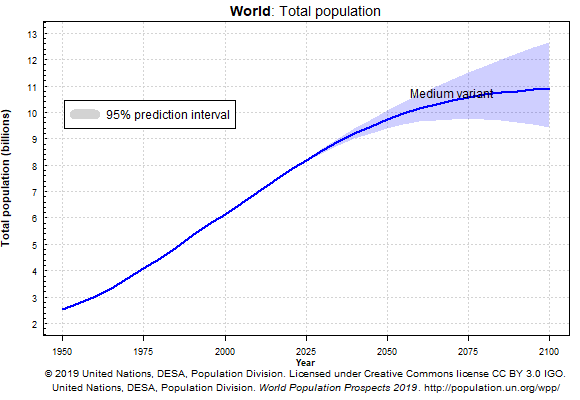
\includegraphics[width=0.8\textwidth]{figures/population.png}
  \caption{Projections for population growth this century \cite{test}} 
  \label{fig:population}
\end{figure}

% Todo: \cite[UN Population Facts] 

Big cities and metropoles around the globe are inevitably growing denser year by year. According to the United Nations, urban areas around the globe have been experiencing an influx of people since the start of industrialization. While the same can be said for rural areas because of the general growth rate of the population, the increase in people moving into big cities is much higher compared to the countryside.
% Todo: \cite[Population Growth in the World's Largest Cities]
% Todo: \cite[UN Interactive Data: Annual Urban Population at Mid-Year (thousands)]
% Todo: \cite[UN Interactive Data: Annual Rural Population at Mid-Year (thousands)]
% Todo: \cite[UN Interactive Data: Average Annual Rate of Change of the Urban Population (percent)]
% Todo: \cite[UN Interactive Data: Average Annual Rate of Change of the Rural Population (percent)]
Depending on how certain factors evolve, such as climate change, autonomous driving, and other technology and politics, it could decelerate or even accelerate growth.

To solve issues stemming from the increased demand in housing, traffic, and infrastructure, urban planning is one of the most important tools. Improving traffic control requires knowledge of the traffic flow and inefficiencies that are causing traffic jams. Knowing local population trends, movement patterns, and other factors could benefit the planning of housing and energy infrastructure. There are only a handful of companies that hold the monopoly on the much-required data, but acquiring them is expensive and can cause problems with data protection laws. Publicizing the information without anonymizing it, severely infringes on the privacy of the originator of the data. But the sole act of anonymizing the data is often not enough. The use of inference attacks may make it possible to associate data and re-identify the individual, as Sweeney has proven.
% Todo: \cite[k-Anonymity/ A Model for Protecting Privacy]

To solve some of the issues, we can leverage the widespread availability of portable computing power, and create a platform that provides the data on a need-to-know basis. Today, most smartphones are equipped with several sensors, including a GPS sensor, pedometer, and accelerometer, which can be used to collect a wide variety of mobility data. Many applications are already utilizing those sensors to implement location-based services and games; for instance, Google Maps, Uber, and Pokemon GO. But there has been a lot of controversy around products of that kind. "If you're not paying, you're the product" is a quote that is often cited around data-driven applications.
% Todo: \cite[https://www.nytimes.com/2018/04/08/us/facebook-users-data-harvested-cambridge-analytica.html]
% Todo: \cite[https://www.ted.com/talks/zeynep_tufekci_we_re_building_a_dystopia_just_to_make_people_click_on_ads]
% Todo: \cite[https://arstechnica.com/tech-policy/2018/04/steve-wozniak-leaves-facebook-the-profits-are-all-based-on-the-users-info/]
It applies to a lot of free services offered in exchange for your data. Google Maps, for example, provides a free navigation service, while collecting your sensory data, such as GPS and accelerometer, staying informed about traffic information. Facebook provides a free social media platform for people to connect, in turn, using collected data to sell targeted advertising.

How they use your data is not in your control. So publicizing big anonymous data sets has its limits, and data collection itself is a hot topic in today's media. 

Simon van Endern proposed a solution to return control over the data back to the users. He implemented a platform that used the power of crowdsourcing the data collection and aggregated the data on a central server on request. \cite{simon}
% Todo: \cite[Simon van Endern]

\section{Research Questions}
When collecting data, it is crucial to find a balance between its usability and the privacy of the collecting party. It is also important to keep in mind, that there has to be a level of trust in both the data collector and the data analyst.
\subsection*{RQ1: What are the benefits and drawbacks in Simon van Endern's architecture and what improvements are possible?}
We take a look at Simon van Endern's original idea and implemented architecture. His work lays a great foundation to create a crowdsourcing platform to collect data while protecting the privacy of its users. We will investigate both the advantages and disadvantages of his idea in regards to scalability, security, and privacy. His work shows a minimal viable product on which we can expand further. We will inspect the choices for the design of the Android app and its data collection. We will also take a look at the data flow of the data aggregation and try to locate inefficiencies and deficits and find solutions to the problems.
\subsection*{RQ2: What information do the raw values for steps and activities reveal?}
As Simon van Endern has shown, mean values expose less private information. We will go into the raw data that make up the mean values and analyze the privacy concerns regarding the distribution of the step values and activities values for the participants and if they can be used to link to other data.
\subsection*{RQ3: How much information does the aggregation of real location data expose?}
Related work has shown that location data are very susceptible to leaking private information. We will try to find ways to collect GPS data and aggregate them without leaking sensitive data. We will research methods to disassociate the mobility data with the individual to provide privacy or anonymity while maintaining statistical relevance.
\subsection*{RQ4: Can we use the current state of P2P technology to remove intermediate third parties?}
In Simon van Endern's implemented platform, he uses a central server to communicate with all devices. There have been a lot of advancements in direct communication frameworks, and we will checkout possible SDKs that can be leveraged to implement and enable a more decentralized and/or distributed architecture.

\section{Contributions}
Our research has the same structure as Simon van Endern's. He has already laid the groundwork with his bottom-up approach of collecting mobility data using crowdsourcing and the aggregation of some basic data. Similarly, raw data is only stored on the devices on which it is generated and only used to aggregate into a larger data set without identifiers. If necessary, the aggregated data set will be processed to anonymize it before publishing it. Using his idea, we will expand into the aggregation of real location data and analyze them for privacy risks with a field test and a simulated one.

% Todo: \cite[Simon van Endern]
% Todo: write more content

First, we review related work concerning risks and solutions to sensitive data and pertinent anonymization techniques. After that, we examine Simon van Endern's original idea and his final implementation and expand on his architecture. We propose our approach to solve the  problems mentioned and increase the types of aggregation. Then, we explain the details of our implementation and the design decisions we made. In next chapter, we document our test setups and the deployment and evaluate our collected results for information leaks. Finally, we draw a conclusion on Simon van Endern's and our work and discuss further possible improvements and give instruction on how the project can be reproduced.
